\section{Наблюдения из космоса, особенности и необходимость}

\subsection{Почему он важны?}

\begin{enumerate}
	\item Наблюдения в диапазонах спектра, в которых земная атмосфера непрозрачна. (Можно проводить наблюдения на высотных баллонах и в стратосферных обсерваториях на самолётах. Однако эти способы работают не во всех диапазонах, а также с большими недостатками).
	
	\item Земная атмосфера существенно влияет на качество изображения (системы адаптивной оптики спасают не от всего), поэтому даже небольшие телескопы, выведенные в космос, позволяют получать принципиально более качественные изображения ярких объектов.
	
	\item В космосе мы не ограничены ни кривизной поверхности, поэтому можно создавать установки очень большого размера.
	
	\item В космосе всегда хорошая погода. (На Земле может случиться так, что во время интересного события погода плохая во всех обсерваториях, это маловероятно, но реально)
	
	\item Для наблюдений доступно всё небо.
\end{enumerate}

\subsection{Поглощение в атмосфере}

Земная атмосфера не очень прозрачна (см. рисунок \ref{fig:2_atmosphere}), однако есть окна прозрачности. Самые большие их них: в радио диапазоне, в оптическом диапазоне. Ультрафиолет и рентген поглощаются полностью. 
Обсудим те диапазоны, которые  не подходят для наблюдения с поверхности Земли.

\begin{figure}[H]
	\centering
	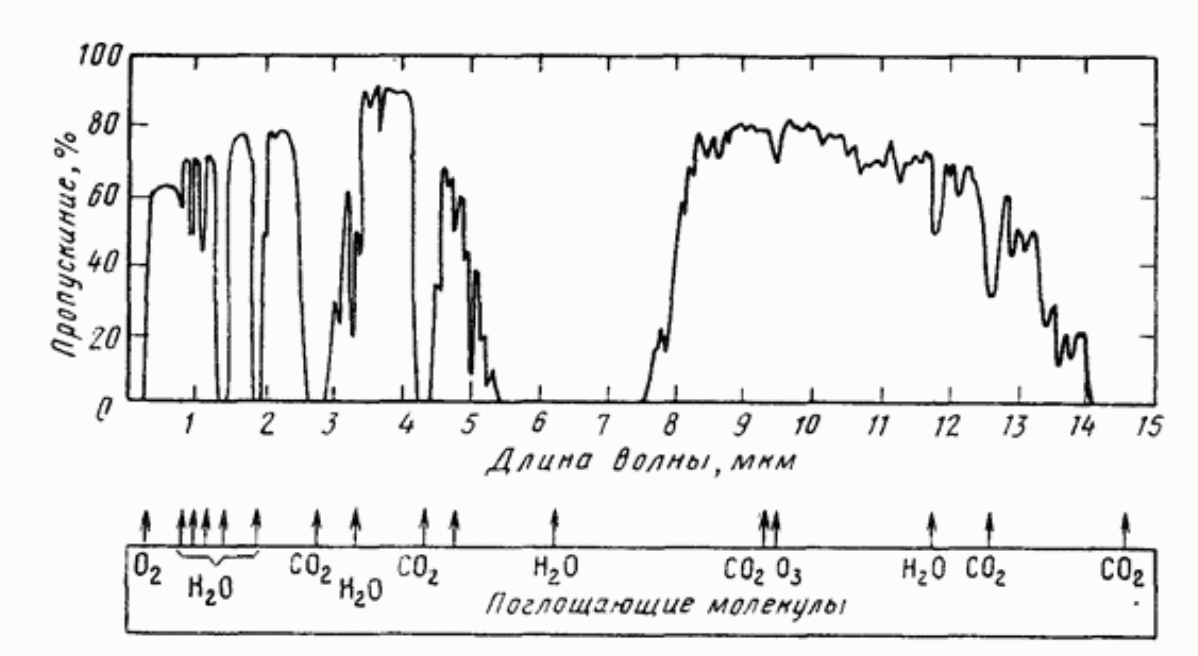
\includegraphics[width=0.7\linewidth]{2_atmosphere}
	\caption{Прозрачность земной атмосферы}
	\label{fig:2_atmosphere}
\end{figure}

\subsubsection{Гамма-астрономия в космосе}

Некоторая часть этого диапазона не доступна для наблюдений с Земли. Это самое жёсткое излучение. Гамма-диапазон – первый диапазон, освоенный астрономами в космосе. Первый астрономический спутник (Explorer 11) имел очень простые детекторы гамма-излучения.

Комптоновская гамма обсерватория: 4 прибора под разные участи этого диапазона. 

Сейчас на орбите находится обсерватория Fermi. 

Точность определения координат в этом диапазоне не очень велика.

Гамма телескопы  не совсем являются телескопами, так как мы не умеем фокусировать лучи (они или проходят сквозь, или слишком легко поглощаются при взаимодействии с веществом, а вот отражаются плохо…). Из-за этого по принципу устройства установки больше похожи на детекторы частиц (см. рисунок \ref{2_fermi_lat}). По траекториям электронов и позитронов удаётся определять направление прилетающих  гамма квантов. Таким образом, направление на источник определяется по вторичным частицам. Энергия гамма квантов измеряется также косвенно по энергии позитронно-электронной пары.

\begin{figure}[H]
	\centering
	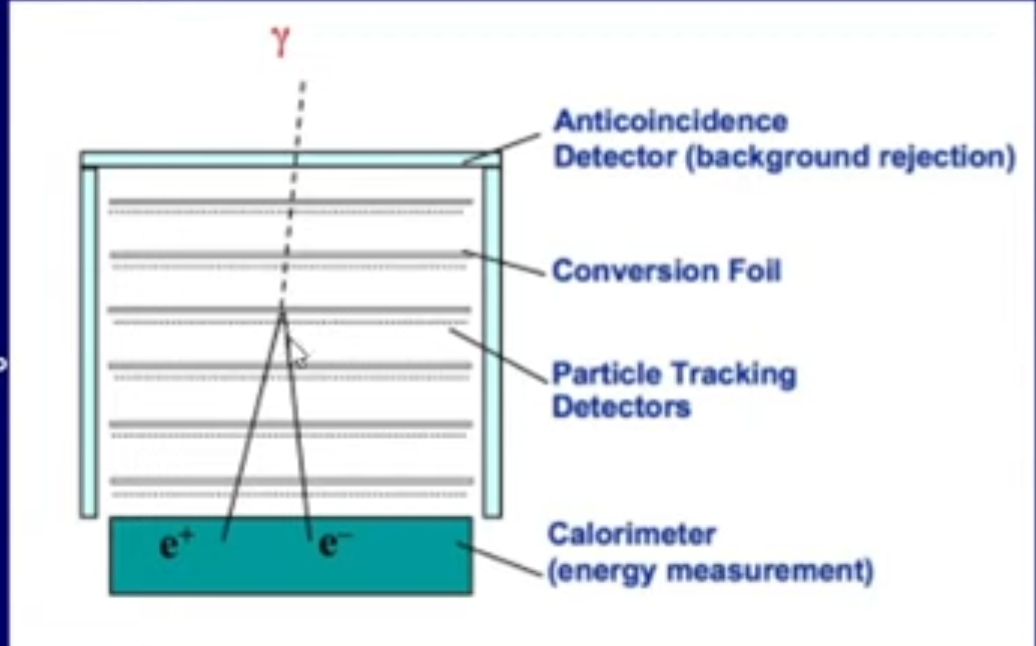
\includegraphics[width=0.7\linewidth]{2_fermi_lat}
	\caption{Ферми LAT}
	\label{fig:2_fermi_lat}
\end{figure}

\subsubsection{Рентгеновская астрономия}

\begin{itemize}
	\item Первые рентгеновские телескопы тоже были детекторами частиц. Сначала измерения проводились ракетами, летевшими по баллистической траектории (то есть время наблюдения очень небольшое). 
	
	\item Первый спутник UHURU (1970) - началась настоящая рентгеновская астрономия. Спутник RXTE, на котором стояли детекторы, которые фиксируют время прихода фотонов. Так как рентгеновских пульсаров очень не много в одном направлении наблюдения, то по периоду прихода фотонов можно определить, сигнал от какого источника получен. (\ref{2_rentgen}) Как происходит регистрация? Есть камера, заполненная газом. Есть анод. Пролетает ионизирующая частица (в данном случае это квант рентгеновского излучения).  Летящая частица выбивает электроны, которые начинают двигаться к аноду. Но поданное напряжение ускоряет электроны, которые начинают выбивать другие электроны…Таким образом, результирующий сигнал усиливается, после чего мы измеряем ток, его легче регистрировать.
	
	\begin{figure}[H]
		\centering
		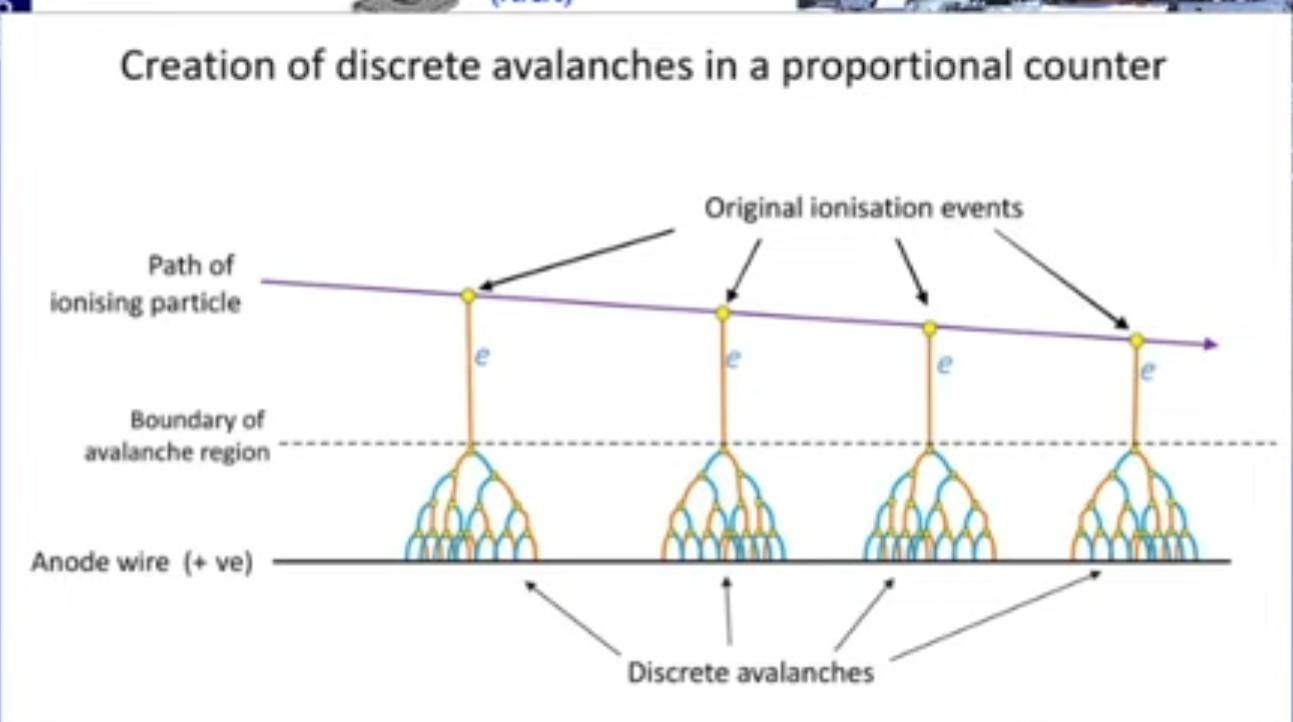
\includegraphics[width=0.7\linewidth]{2_rentgen}
		\caption{К методу работы рентгеновской астрономии}
		\label{fig:2_rentgen}
	\end{figure}
	
	\item Кодирующие маски. Отражений и преломлений всё ещё нет, но мы делаем шаг вперёд: улучшаем пространственное разрешение.  Теперь лучше понимаем, откуда прилетела частица. Реализовано на спутнике Integral. Кодирующая маска: сложная затемняющая картина (см. рисунок \ref{fig:2_code_mask}). Если мы будем смотреть на тени от источников, то тени будут достаточно причудливыми, поэтому будет легко  определять, где находятся источники. Улучшено угловое разрешение.
	
	\begin{figure}[H]
		\centering
		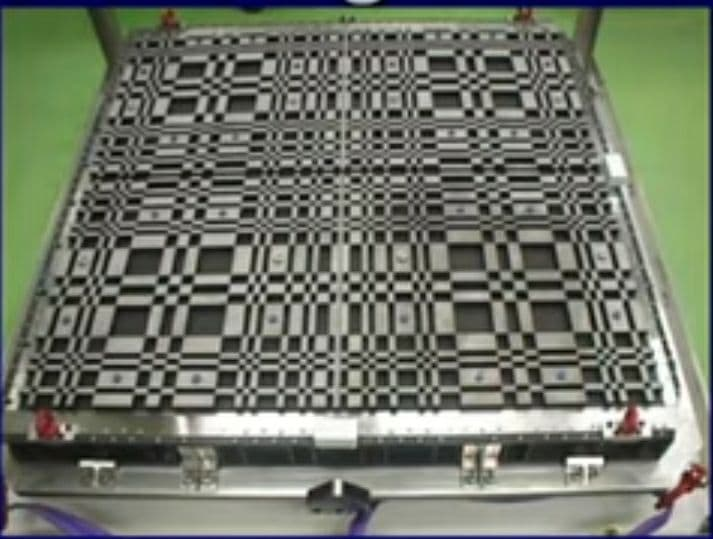
\includegraphics[width=0.7\linewidth]{2_code_mask}
		\caption{Кодирующая маска}
		\label{fig:2_code_mask}
	\end{figure}
	
	\item Современная рентгеновская астрономия. Появилась фокусирующая оптика. В 1979 году был запущен первый такой прибор. Сейчас на орбите два таких инструмента (Chandra и XMM-Newton). Как работает фокусировка? Зеркала косого падения. Рентгеновские кванты отражаются, но плохо. (Аналогия: можно бросить в воду кирпич, и он утонет, то есть не отразится. Можно бросить камень под очень маленьким углом к поверхности, и он будет многократно отражаться). Так и здесь: создаётся вложенная система зеркал, от каждого из которых отражение происходит под малым углом (см. рисунок \ref{fig:2_reflect}). Запускать такие телескопы сложно, так как система требует соосности зеркал с хорошей точностью.
	
	\begin{figure}[H]
		\centering
		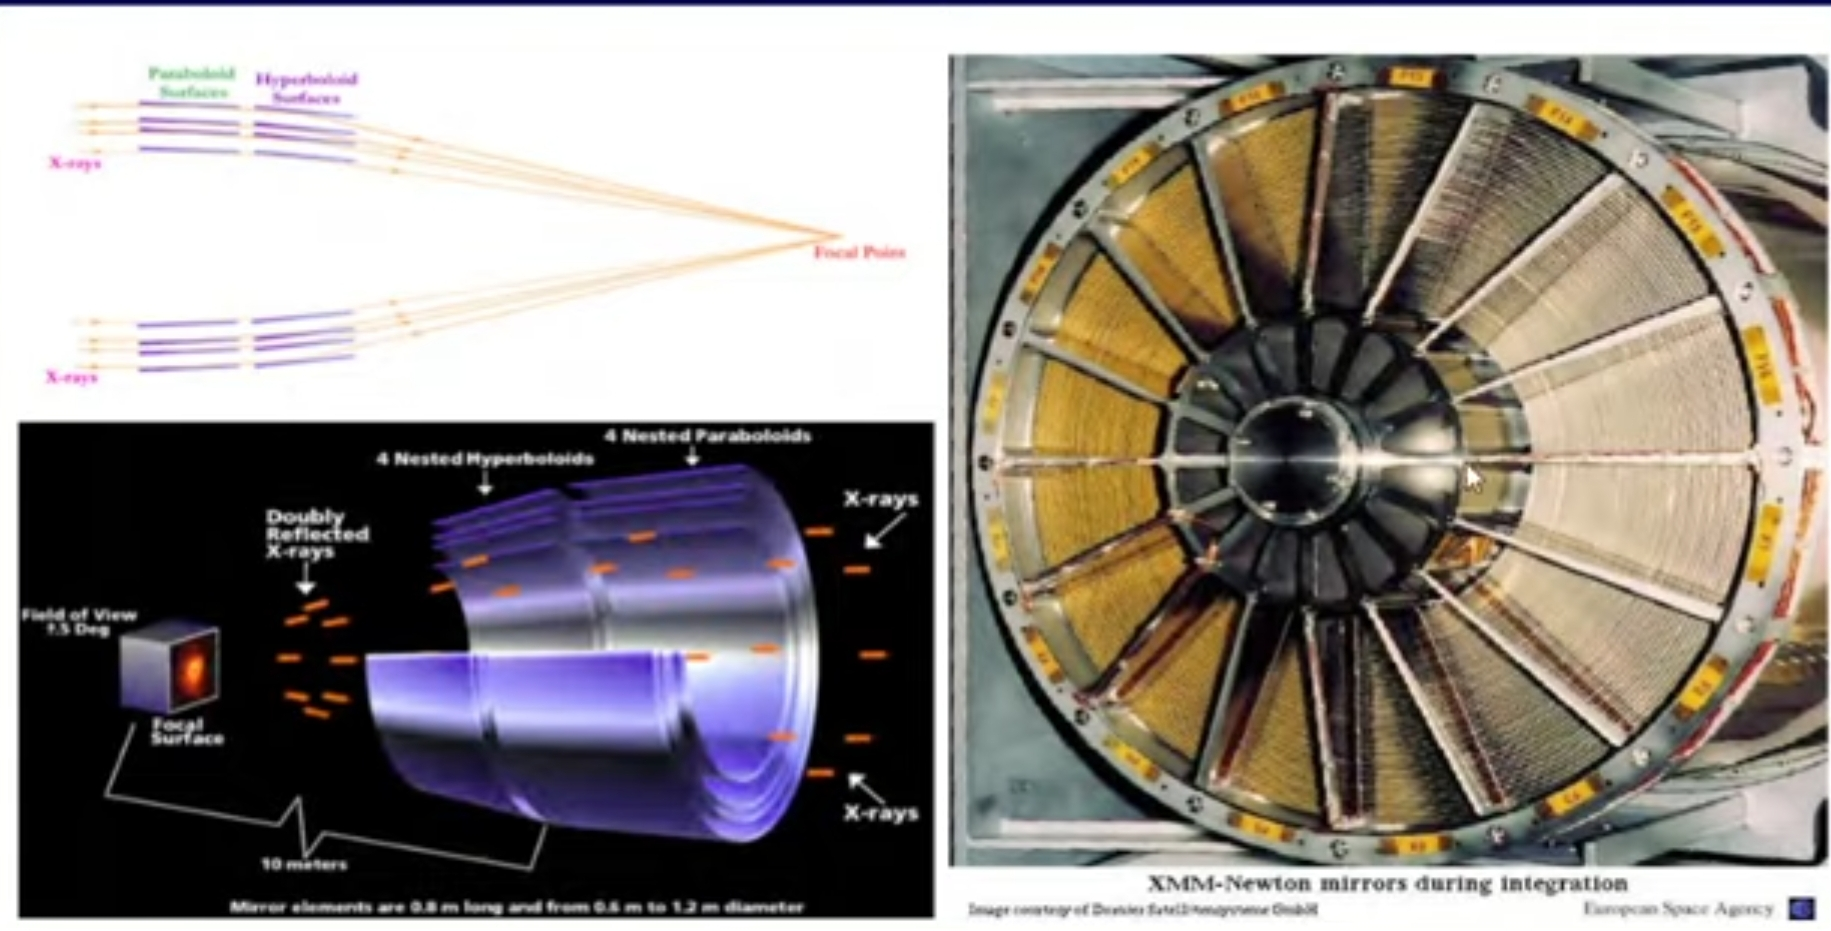
\includegraphics[width=0.7\linewidth]{2_reflect}
		\caption{Вложенная система зеркал}
		\label{fig:2_reflect}
	\end{figure}
	
	\item Идём в более короткие волны, т.е. угол падения должен быть ещё меньше, из-за чего система становится ещё длиннее, а это сложно. Решение: система  NuSTAR. Спутник состоит из двух частей. Отдельно летает оптика, и на расстоянии в несколько десятков метров от неё летает блок приёмной аппаратуры. Но это требует фантастической синхронизации. NuSTAR – раскладывающийся спутник (см. рисунок \ref{fig:2_NuSTAR}).
	
	\begin{figure}[H]
		\centering
		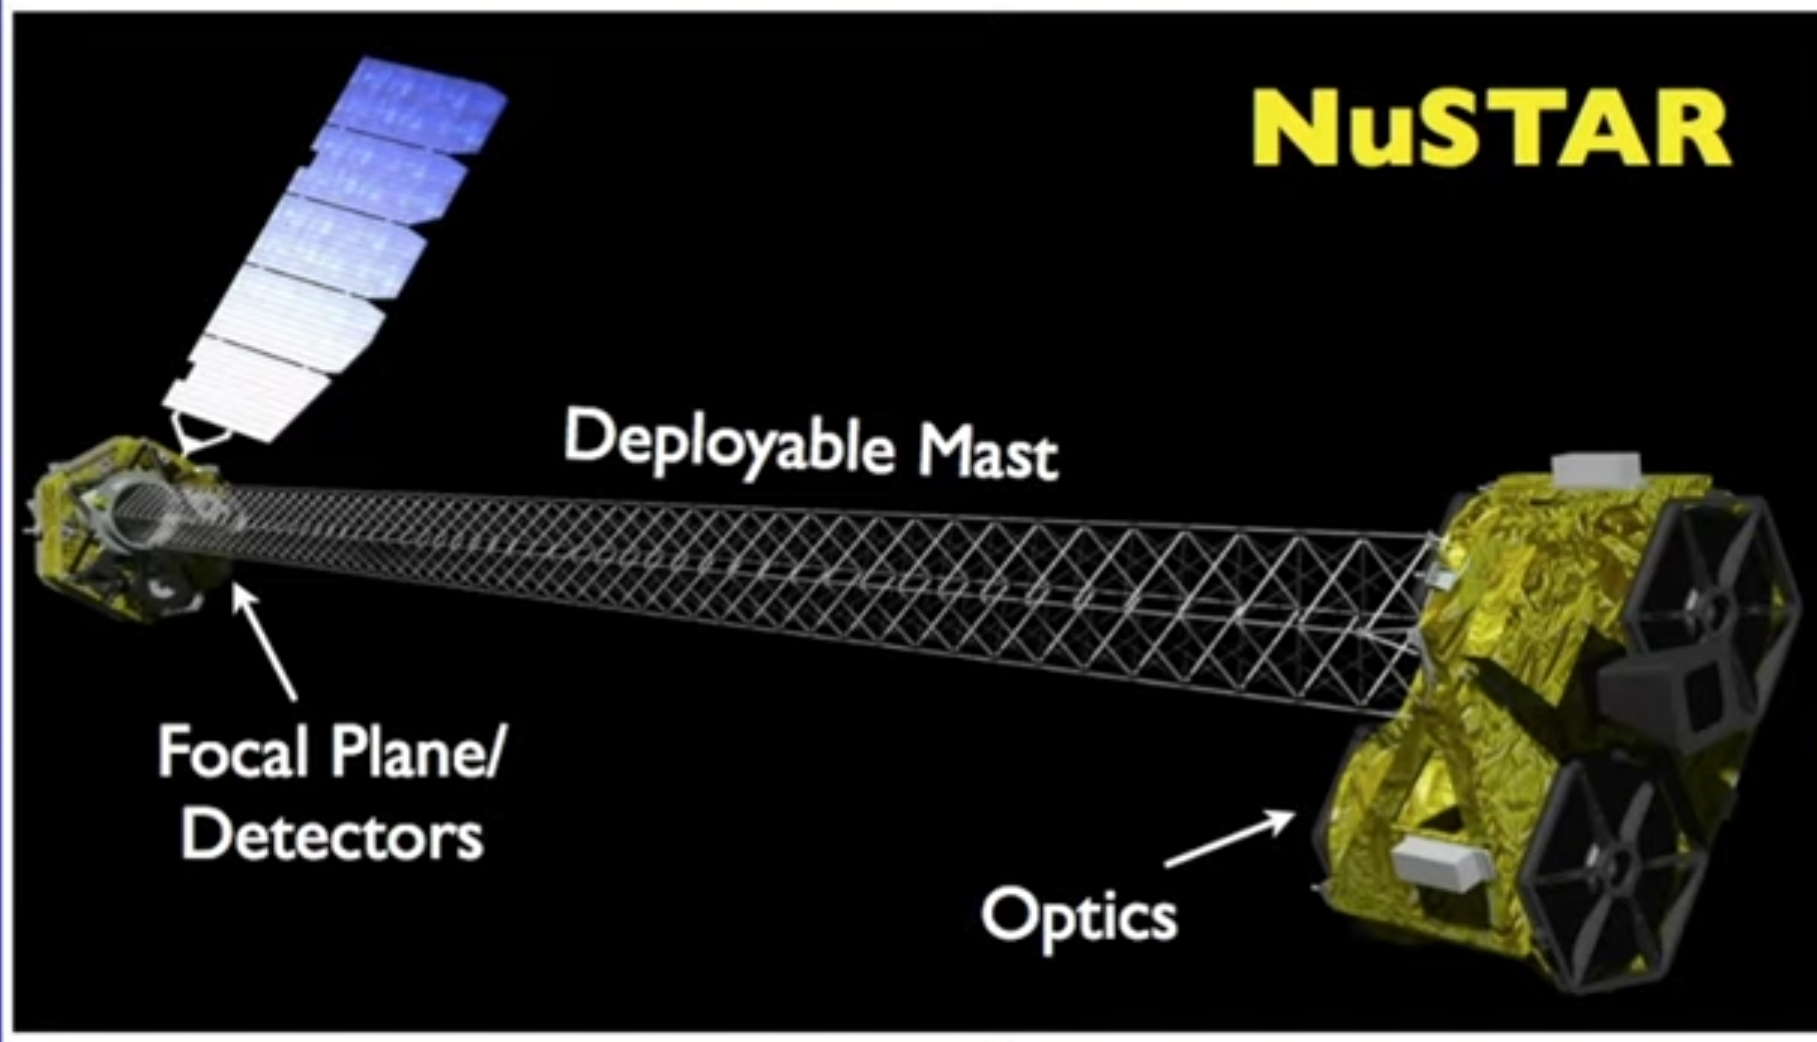
\includegraphics[width=0.7\linewidth]{2_NuSTAR}
		\caption{Спутник NuSTAR}
		\label{fig:2_NuSTAR}
	\end{figure}
\end{itemize}

\subsubsection{Инфракрасная астрономия}

Многие астрофизические процессы лучше наблюдать в ИК диапазоне, например, рождение звёзд и планет. Пример телескопа – «Спитцер».

С зеркалами тут всё проще, нам подходят привычные зеркала (почти как в оптическом диапазоне). При этом качество зеркало должно соответствовать длине волны, т.е. не требуется безумное качество поверхности. Однако есть проблема: всё вокруг излучает в этом диапазоне, даже люди! Чтобы решить эту проблему нужно охладить почти весь спутник жидким гелием, кроме того, нужно закрыть систему от Солнца специальным экраном. Но экран будет нагреваться и излучать…Эту проблему тоже надо решать. \textbf{Срок жизни спутника ограничен запасами жидкого гелия}. Но после исчерпания запасов жидкого гелия можно использовать телескопы в качестве неплохих в оптическом диапазоне.

Из интересных результатов в этом диапазоне: телескоп «Спитцер» смог восстановить карту распределения температуры по видимой поверхности планеты.

\subsubsection{Астрономия в оптическом и прилегающих диапазонах}

Телескоп имени Хаббла. Его диаметр всего 2.4 метра, однако он получил много важных результатов, так как ему не мешает атмосфера + длинные экспозиции. Он может строить изображения и получать спектры в видимом, ИК и УФ диапазонах. Способен наблюдать объекты до 31 звёздной величины.

Приборы Хаббла: некоторое время к нему можно было летать, поэтому несколько раз привозили современную аппаратуру. 

\medspace

\textbf{Астрометрические наблюдения}. Она тоже используют преимущества наблюдений из  космоса:  Gaia. Открытие экзопланет. Тут тоже мешает атмосфера.

\textbf{Большие установки}. Интерферометр на гравитационных волнах. Космический проект eLISA. 

\textbf{Космические лучи}. Изучение редких частиц высоких энергий. Находясь снаружи, мы можем наблюдать сразу за ~ половиной атмосферы Земли.

\textbf{Обзоры}. Можно «отсмотреть» всё небо одним прибором, а не «склеивать кусочки». С поверхности планеты так сделать нельзя. Например, нужно смотреть за реликтовым излучением именно на всём небе. Спутник Plank следил за реликтовым излучением.

Кроме того, может понадобиться постоянный мониторинг всего неба. Например, следим за потенциально опасными астероидами.



